%% \abstract{When a listener hears many good examples of a /b/ in a row, they are less likely to classify other sounds on, e.g., a /b/-to-/d/ continuum as /b/.  This phenomenon is known as \emph{selective adaptation} and is a well-studied property of speech perception.  Traditionally, selective adaptation is seen as a \emph{mechanistic} property of the speech perception system, and attributed to fatigue in acoustic-phonetic feature detectors.  However, recent developments in our understanding of non-linguistic sensory adaptation and higher-level adaptive plasticity in speech perception and language comprehension suggest that it is time to re-visit the phenomenon of selective adaptation.  We argue that selective adaptation is better thought of as a \emph{computational} property of the speech perception system.  Drawing on a common thread in recent work on both non-linguistic sensory adaptation and plasticity in language comprehension, we furthermore propose that selective adaptation can be seen as a consequence of \emph{distributional learning} across multiple levels of representation.  This proposal opens up new questions for research on selective adaptation itself, and also suggests that selective adaptation can be an important bridge between work on adaptation in low-level sensory systems and the complicated plasticity of the adult language comprehension system.}



\chapter{Re-examining selective adaptation: Fatiguing feature detectors, or distributional learning?}\label{chap:selective-adaptation}


Repeated exposure to a prototypical example of a phonological category seems to `shrink' that category. For example,  exposure to a reasonably good example of a \ph b many times in a row makes listeners less likely to classify other sounds on a \ph b-\ph d continuum as \ph b \autocite{Eimas1973}.  The discovery of this effect, known as \emph{selective adaptation}, led to a great deal of excitement among speech perception researchers.
By analogy with similar adaptation effects in visual psychophysics, it promised a ``psychophysicist's microelectrode'' \autocite{Frisby1979,Mollon1974}, a powerful and general method of probing the neural code by which continuous acoustic input is transformed into discrete linguistic units, and hence potentially resolving fundamental debates about the psychological reality and properties of phonemes and phonetic features hypothesized by formal linguistic analysis.  Selective adaptation effects in visual perception, for instance, were critical in establishing---based on behavior alone---the features used by the visual system to analyze visual input \autocite[e.g.,][]{Blakemore1969}, and it was hoped that the same sort of effects in speech perception would be able to establish the existence of feature detectors for abstract linguistic categories like phonemes and phonetic features like \emph{voicing}.
But this excitement was quickly tempered for a variety of reasons.  Chief among them were findings suggesting that selective adaptation reflects something more like fatigue of general sensory feature detectors, rather than \emph{language-specific} processing of speech sounds \autocite[e.g.,][]{Remez1979,Samuel1979,Schouten1980,Roberts1981}.  \label{r-fd1} More deeply problematic, the patterns of adaptation observed were not consistent with fatigue of the \emph{kind} of feature detectors that had been assumeed \autocite[see][for an excellent critique]{Remez1987}.  It became clear that adaptation effects needed to be explained as phenomena in their own right, and subsequently selective adaptation fell out of favor in work on speech perception \autocite[cf.][]{Remez1987,Samuel1986}.

In the decades since the rapid rise and fall of selective adaptation, we have learned a great deal about adaptive properties of sensory systems generally, and speech perception in particular.  We argue that taken together, these bodies of work suggest that it is time to re-examine the phenomenon selective adaptation.
Two developments contribute to our argument. 
First, recent work challenges the idea that sensory adaptation is best thought of as the fatigue of feedforward feature detectors, or more broadly as a \emph{mechanistic} property of sensory systems. Rather, an emerging perspective views adaptation as a \emph{computational} property of sensory systems, where the sensitivity of the sensory system (with its limited neural resources) is re-aligned to information that is relevant to the task at hand and meaningful in the current environment \autocite[e.g.,][]{Gutnisky2008,Kohn2007,Stocker2006,Webster2005}.  While in some cases this re-alignment might be achieved by detector fatigue, there is a growing body of work that cannot easily be accounted for in this way (which we will discuss below).  Second, the last decade of speech perception research has revealed that, far from a series of fixed feature detectors, the speech perception system is adaptive and flexible in smart ways \autocite[e.g.,][]{Bertelson2003,Bradlow2008,Clayards2008,Kraljic2008a,Maye2008a,Norris2003}.  Plasticity and context-sensitivity are increasingly understood to be central features of a speech perception system that has to function in a world where the cue-to-category mapping depends on aspects of the local environment, like \emph{who} is talking \autocite{Norris2003,Huang2012,Laing2012}.

These developments, we argue, undermine two of the basic assumptions of early work on phonetic selective adaptation: that speech perception is (1) performed by acoustic-phonetic feature detectors that (2) become fatigued if they are stimulated too often.  
\label{r-fd2} In this paper, we focus on the fatigue assumption \autocite[see][for a rejection of the feature detector assumption]{Remez1987}.  In part, we focus on fatigue because contemporary speech perception research views selective adaptation as a fatigue effect that is qualitatively different from other sorts of plasticity \autocite[e.g.,][]{Grabski2013,Vroomen2004,Vroomen2007,VanderZande2014,Zaske2013}.
More importantly, we focus on fatigue here because the developments mentioned above do more than just undermine the fatigue assumption.  Additionally, we propose, they provide a productive lens through which to re-examine the phenomenon of selective adaptation, and speech perception more generally.

A common thread that runs through recent work on sensory adaptation and flexibility in language comprehension is the idea of \emph{distributional learning} across \emph{multiple levels}.  The sensory information that is relevant or meaningful in the current environment depends on the distribution of sensory features in that environment. Sensory systems adapt to these properties, and to that extent they can be thought of as implicitly learning those distributions \autocite{Brenner2000,Fairhall2001,Gutnisky2008,Sharpee2006,Stocker2006}.  At the same time, building on recent work that treats speech perception as statistical inference \autocite[e.g.,][]{Clayards2008,Feldman2009a,Kleinschmidt2015,Norris2008,Sonderegger2010}, much of the flexibility of speech perception---and language comprehension more broadly---can be seen as a form of distributional learning.  In this view, listeners deal with talker-to-talker variability by updating their beliefs about the distributions of cues (acoustic, phonetic, lexical, etc.) that result when a talker produces a linguistic structure \autocite[phonetic category, word, syntactic structure, pragmatic intention, etc.;][]{Fine2013,Guediche2014,Holt2006c,Idemaru2011,Kleinschmidt2015,YildirimInPress}.

First, we briefly review the evidence that sensory adaptation in general is better viewed as a form of distributional learning, rather than the fatigue of static feature detectors.  Second, we lay out a tentative proposal for how the logic of distributional learning applies to phonetic selective adaptation.  Third, we show that much of the literature on selective adaptation which appears to contradict our proposal is actually \emph{predicted} by it, given a modern understanding of distributional learning that occurs at multiple levels of representation.  Fourth, and finally, we lay out what we see as some of the most pressing questions that this proposal raises for future work.

Our goal is not to show conclusively that selective adaptation \emph{is}, in all cases, distributional learning.  Rather, we hope that distributional learning provides a productive perspective for re-examining previous evidence, and renews interest in selective adaptation as an important phenomenon in need of explanation in its own right, rather than simply a methodological tool.
\label{r-phenomenon}

\section{Sensory adaptation as distributional learning}
\label{sec:sens-adapt-dist-learn}

Non-linguistic sensory adaptation (which usually means visual adaptation) has much in common with phonetic selective adaptation: repeated exposure to a stimulus attribute will reduce responsiveness to that attribute, both at the level of behavior (psychophysics) and neural responses (electrophysiology).  We refer to this decrease in responsiveness as a \emph{negative after-effect}.  For example, after extended viewing of a vertical grating, the contrast threshold for detecting another vertical grating goes up, and the firing rate of neurons in the visual cortex which are sensitive to vertical orientation is reduced when viewing another vertical grating \autocite[cf.][]{Kohn2007}.  These findings were originally explained as fatigue of neuronal populations which are primarily sensitive to the adapted feature \autocite{Blakemore1969}, and when analogous negative after-effects of selective adaptation with speech were first discovered \autocite{Eimas1973}, they too were chalked up to a similar mechanism \autocite[although not without debate, some of which we revisit below; e.g.,][]{Cole1975,Ainsworth1977}.

However, work in the decades since challenges the idea that adaptation is broadly the result of ``dumb'' fatigue of feature detectors \autocite{Kohn2007,Webster2005}.  We now know that adaptation does not just reduce the firing of neurons overall but actually \emph{changes their tuning}, such that some stimuli might even elicit \emph{higher} firing rates after adaptation \autocite{Dragoi2000,Gutfreund2012,Kohn2004}.  Moreover, these changes in tuning have been shown to be coordinated across \emph{populations} of neurons, and often in ways that increase the amount of information that is transmitted about stimuli in the local environment \autocite{Brenner2000,Fairhall2001,Gutnisky2008,Sharpee2006}.  Specifically, changes in tuning seem to serve an increase in the perceptual resolution for the range and distribution of stimuli observed in the current environment (e.g., in an experiment).

This and related findings suggest that selective adaptation has to be understood at least in part as a computational property of sensory systems that need to use limited neural resources to efficiently represent information across a variety of environments \autocite{Brenner2000,Fairhall2001,Gutnisky2008,Kohn2007,Sharpee2006,Wainwright1999,Webster2005}. In order to allocate processing resources, sensory systems need to know, at a basic level, how the features they represent are statistically distributed in the current environment. The sensory information that is most \emph{likely} and \emph{relevant} changes from one environment to the next, and so sensory systems need to adapt to these changes in order to make the best use of their limited neural resources.  One way to distinguish more stimuli using a fixed number of neurons is to change the stimulus features encoded by each neuron's signal based on the current environment, because the environment itself provides some clues as to which stimuli are most likely and how they ought to be interpreted. Viewing adaptation purely as a mechanistic property like feature detector fatigue misses this important point.

How does this computational perspective help to understand the effects observed in a typical adaptation experiment? Consider the extreme deviation such an experiment presents from everyday perception.  The perceptual environments we encounter outside the lab tend to exhibit a lot of variability in stimulus features. In a typical adaptation experiment, however, the exact same stimulus is presented over and over again. This produces a highly concentrated, \emph{non}-variable distribution.  The typical behavioral and neural after-effects of adaptation can be attributed to the retuning of sensory systems to this new distribution, by, for instance, reducing noise or increasing selectivity to make finer-grained distinctions in the more narrow range of stimuli observed in the experiment \autocite{Gardner2004,Stocker2006,Wainwright1999}, or reducing sensitivity to highly predictable stimuli \autocite{Friston2005,Rao1999}.  In order to re-tune itself based on the distribution of sensory features, the sensory system has to, at least implicitly, \emph{learn} those distributions.  In this sense, selective adaptation can be thought of as distributional learning.

Research on selective adaptation in the visual domain provides two pieces of evidence in support of this view that we discuss next.  Both of these phenomena reveal that it is critical to consider distributional learning at \emph{multiple levels}: short-, medium-, and long-term distributions in the first case, and different levels of features (part vs. whole) in the second.

First, to the extent that adaptation is a consequence of distributional learning, stronger adaptation is predicted to occur when the current distribution deviates more from the expected distribution, and more learning is required.
\textcite{Chopin2012} showed that, as predicted by distributional learning, in an (experimental) visual world where right-leaning edges are more common overall, seeing a series a right-leaning bars produces less of a negative after-effect, compared to a world where left-leaning edges are more common. Subjects were asked to say whether a bar was leaning to the left or the right, in a sequence of trials that contained vertical, left-leaning, and right-leaning bars.  Critically, \textcite{Chopin2012} manipulated the short-term and long-term frequency of left- vs. right-leaning trials before each of the vertical test trials.
When there were more right-leaning bars in the short-term history (last 3 minutes), subjects showed the typical negative after-effect, and were more likely to say that a vertical bar was leaning \emph{left}.  But when there were more right-leaning bars in the \emph{long-term} history (from 2 to 10 minutes in the past), subjects showed a \emph{positive} after-effect, and were biased to say a vertical bar was right-leaning.  This effect runs contrary to the basic prediction of the neural fatigue theory of adaptation: more exposure to right-leaning stimuli should \emph{always} result in fewer right-leaning responses, regardless of the long-term statistics of the current environment.


\begin{figure}[!ht]
  \centering
  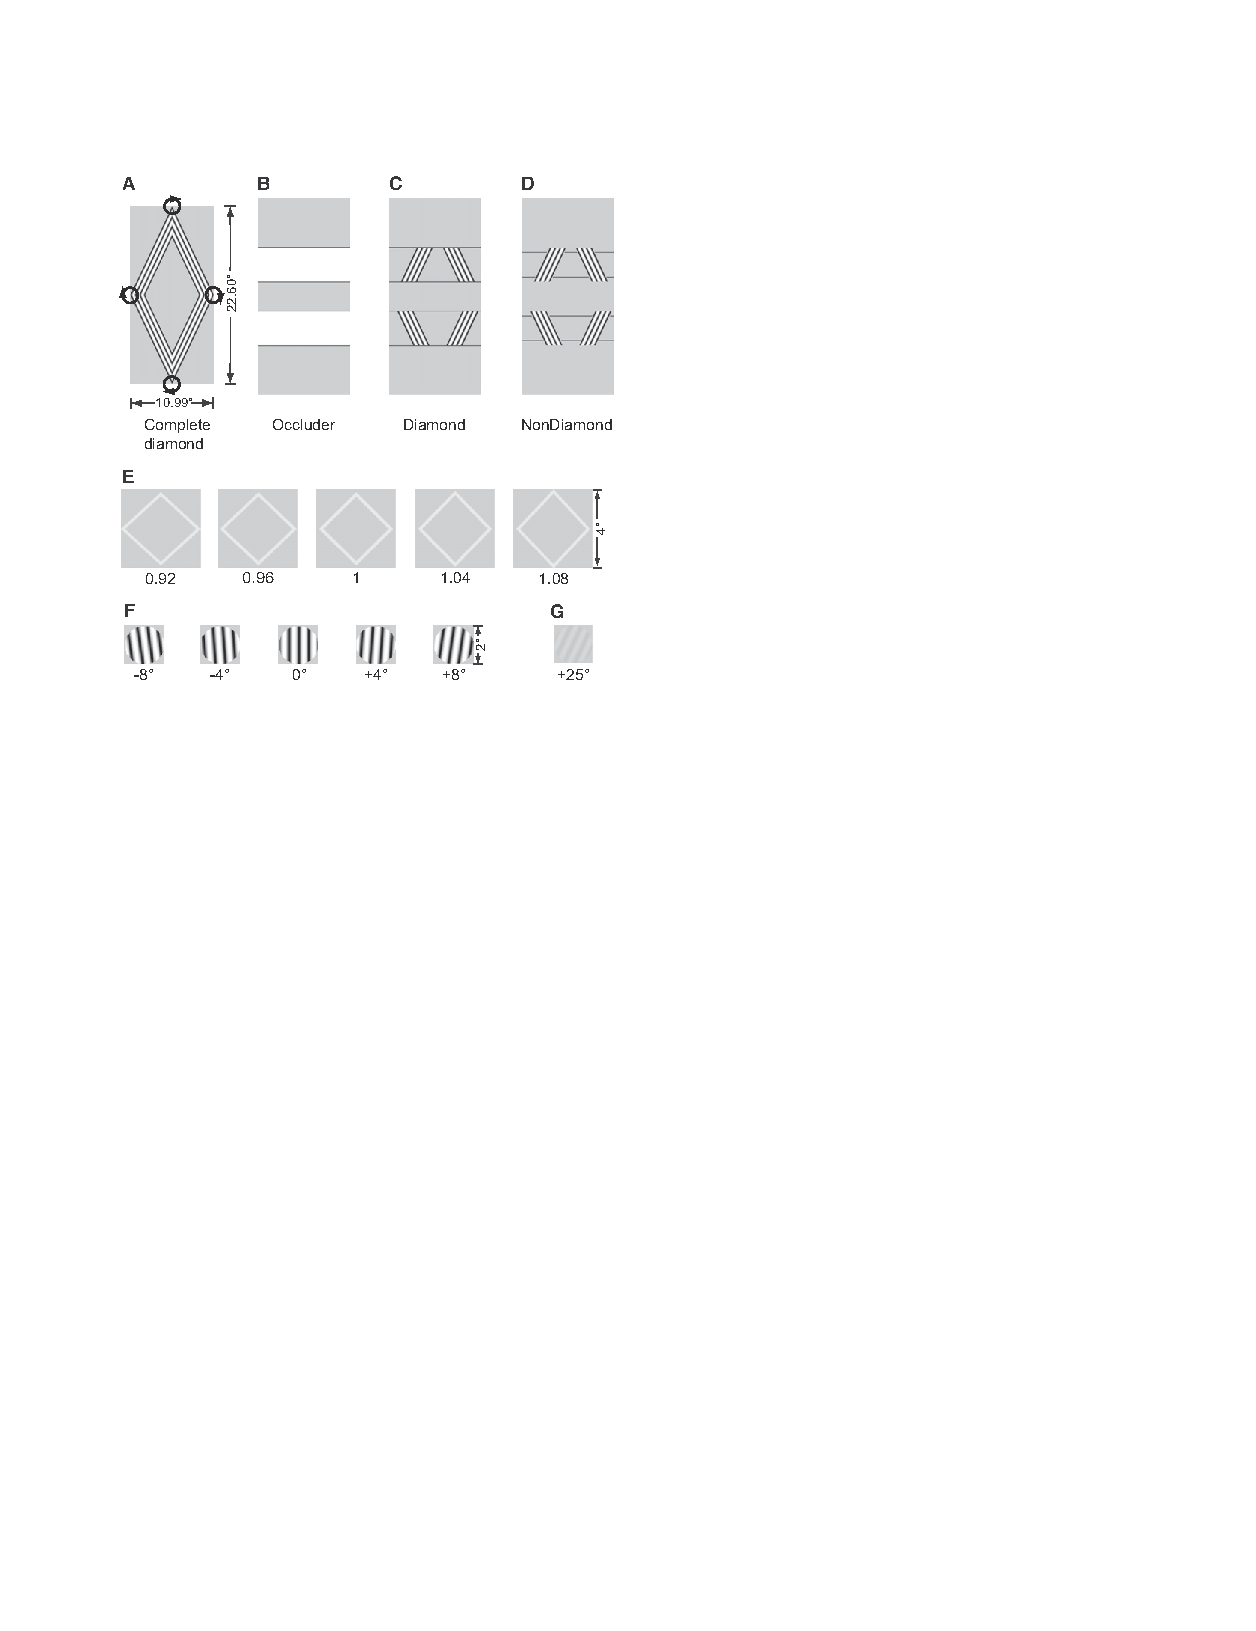
\includegraphics[]{he-et-al-2012-fig1.pdf}  
  \caption{Adaptor and test stimuli used by \protect\textcite{He2012}.  The adaptor stimulus was a diamond shape (A) that rotated behind three occluder bars (B).  In the high-level condition (C), the lines indicating the edges of the occluders matched the portion actually occluded, leading to a percept of a moving diamond shape.  In the low-level condition (D), the lines were moved, leading to a percept of four disconnected edges.  The shape after-effect was tested by means of a tall-versus-wide diamond task (E), while adaptation to the edges themselves was tested via a tilt after-effect, measured with a left-versus-right leaning bar task (F).  Adaptation to the whole shape (C) produced strong shape after-effects (E) but much weaker tilt after-effects (F) than the non-fused edges (D).  Figure reproduced with permission from He et al. (2012).}
  \label{fig:he-et-al-2012-stims}
\end{figure}

Second, high-level features can change the expected distribution of lower-level features, and distributional learning predicts that such a change should lead to more or less adaptation to those lower-level features.  For instance, the presence of a diamond shape predicts the presence of oriented bars corresponding to its edges.  Sensory adaptation indeed appears to be sensitive to this dependence as well: adaptation to a higher-level feature---like a shape---reduces or eliminates the after-effects produced by its component features---like individual edges---when presented in isolation \autocite{He2012}.
By manipulating perceptual grouping of individual oriented bars, \textcite{He2012} changed whether they were perceived as edges of a single figure (a diamond, Figure~\ref{fig:he-et-al-2012-stims}, C) or as separate objects (four bars, Figure~\ref{fig:he-et-al-2012-stims}, D).  When the bars were perceived as separate, each feature individually produced the typical after-effect.  However, when all of the features were perceptually grouped into a diamond, the after-effects of the individual features were substantially reduced.  Instead, a higher-level \emph{shape} after-effect was obtained.  Again, this effect runs contrary to a fatigue theory of adaptation.  Subjects were exposed to exactly the same low-level features in both cases (edges with the same orientation). Thus the corresponding edge detectors should be subject to the same fatigue.  But only when there is no higher-level feature that explains the oriented edges is there any adaptation to the oriented edges themselves.

In both of these cases, attributing selective adaptation to fatigue fails to explain the observed effects. Distributional learning, however, offers a possible explanation. In a distributional learning theory of adaptation, negative after-effects happen because the sensory system has adjusted to an unusual distribution of stimuli.  The degree of adjustment, and hence the strength of the negative after-effects, is determined by just how unusual that stimulus distribution is, compared to what is typical or expected.  Critically, a stimulus distribution that would be highly unusual on its own might be perfectly typical if it is similar to the distributions encountered in medium-to-long-term history \autocite[e.g., as in][]{Chopin2012} or predictable given the presence of higher-level features \autocite[e.g., as in][]{He2012}.  To a first approximation, a distributional learning theory thus correctly predicts that such \emph{predictable} or \emph{expected} deviations in sensory statistics should produce weaker after-effects than unpredictable deviations.\footnote{An important caveat is that if the statistics deviate \emph{too} much from what is expected, then learning may not be possible at all.  One notable example from speech perception is that listeners do not adapt fully to highly unusual accents \protect\autocite[e.g.,][]{Idemaru2011,Sumner2011}.}

A growing body of evidence thus suggests that non-linguistic sensory adaptation is intimately tied to the distribution of sensory features in the current environment.
Rather than inducing the same adaptation regardless of the environment, the effect of repeated exposure to low-level features depends on higher-level statistics of the environment. 
This work shows that the distribution of sensory features in isolation are not enough for understanding adaptation.  Rather, it is necessary to consider sensory feature distributions across \emph{multiple levels}, both in the sense of part-whole feature relationships \autocite{He2012} and in the sense of short-, medium-, and long-run distributions of a single feature \autocite{Chopin2012}.
Next, we review how the same distributional learning logic can be applied to selective adaptation in speech perception.


\section{Phonetic selective adaptation as distributional learning}
\label{sec:select-adapt-as}

At the most basic level, the distribution of acoustic cues determines the mapping from acoustic cues to the underlying phonetic categories.  Moreover, these distributions can vary quite a bit from one talker to the next.  This variability means that in order to robustly recognize phonetic categories, the speech perception system must, in some way, be sensitive to changes in these statistics \autocite{Kleinschmidt2015,McMurray2011a}.  One way of achieving this sensitivity is by distributional learning
\autocite[for a review of additional means, such as normalization, see][]{WeatherholtzInPress}. 
Indeed, research on speech perception has accumulated an impressive body of evidence that adult listeners do engage in distributional learning during speech perception, both at the level of cues \autocite[e.g., recalibration/perceptual learning,][]{Bertelson2003,Clayards2008,Feldman2013b,Kraljic2007,Munson2011,Norris2003} and at the level of phonetic categories themselves \autocite[e.g. learning novel phonotactic constraints,][]{Dell2004,Warker2006,Warker2009}.  Recent work further suggests that adults also engage in distributional learning at higher levels of linguistic representation, like syntactic structures \autocite{Chang2006,Fine2013,Jaeger2013a,Kamide2012} and pragmatics \autocite{Kurumada2014,Kurumada2012,YildirimInPress}.  As with general sensory adaptation reviewed above, this learning seems to be a form of ``smart'' plasticity that increases the speed and accuracy of language processing in the face of uncertainty and variability across environments \autocite[for review, see][]{Kleinschmidt2015}.

\begin{figure}[ht]\centering
  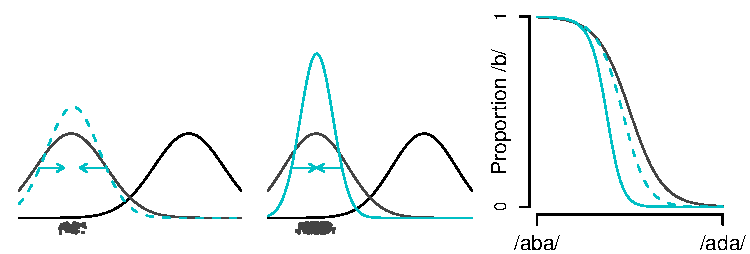
\includegraphics[width=\textwidth]{schematic-adapt.pdf}
  \caption{Distributional learning accounts for the negative after-effects observed in phonetic selective adaptation.  Repeated exposure to a prototypical \ph b results in a distribution with much lower variance than normal (left).  Learning this distribution means that previously ambiguous stimuli are now, to the listener, more likely to be occur if the intended category was \ph d, resulting in a negative shift in the \ph b-\ph d category boundary (right).  Incremental belief updating predicts that the more exposure to this distribution the listener has, the more their beliefs should reflect it (left vs. middle) and the stronger the after-effect (right, dashed vs. solid).}
  \label{fig:schematic-selad}
\end{figure}

Distributional learning in speech perception is a prerequisite for a distributional learning account of selective adaptation, but how does the logic of distributional learning play out for selective adaptation to phonetic input?  Intuitively, the logic is the same as for adaptation in the visual domain, discussed above.  Consider a typical phonetic adaptation experiment, where a listener hears a prototypical \ph b repeated over and over again.  This leads to a very odd distribution of acoustic cues: typically, there is some variability in the signal, even when the same category is repeated by the same talker in the same phonological context \autocite{Allen2003,Newman2001}.  Such a highly concentrated distribution might, intuitively, correspond to a talker who is \emph{very} precise in how they produce their \ph bs.  Such a talker is less likely to produce a \ph b with a cue value that, for a normal talker, would be ambiguous between a \ph b and a \ph d.  Consequently, if the listener has learned this changed distribution, then we would predict that they classify fewer items by the same talker on a \ph b-to-\ph d continuum as \ph b (Figure~\ref{fig:schematic-selad}).

This reduction in \ph b responses after \ph b exposure is exactly the negative after-effect (shift in category boundary) that characterizes selective adaptation in speech \autocite{Eimas1973,Samuel1986}.  Thus, qualitatively, distributional learning provides an account for selective adaptation, at least as far as its effects on classification are concerned.  Quantitatively, too, distributional learning provides a good fit against data from selective adaptation: the incremental effects of repeated exposure to the same stimulus are well-described by a distribution learning model \autocite[$r^2=0.85$,][]{Kleinschmidt2015}. 

\label{r2-whole-distribution-1}
The ``ideal adapter'' distributional learning model developed in \textcite{Kleinschmidt2015} predicts that listeners do not just track the variance of cue distributions, but the \emph{whole} distribution, which includes at least both the \emph{means} and variances of cue distributions.  The same model can be applied to phonetic recalibration/perceptual learning, where listeners hear an {\em a}typical production of \ph b which is acoustically ambiguous between \ph b and \ph d, but which is disambiguated by, e.g., a visual cue or lexical context.  The resulting cue distribution is unusual both in terms of its mean and its variance.  Recalibration is characterized by a \emph{positive} after-effect: after such exposure, listeners classify \emph{more} items from a \ph b-\ph d continuum as \ph b.  Recalibration, unlike selective adaptation, has traditionally been described as a form of implicit learning \autocite{Norris2003,Vroomen2004,Vroomen2007}.  Nevertheless, the very same distributional learning model fits listeners' classification behavior in a recalibration experiment just as well as for selective adaptation \autocite[$r^2 = 0.86$,][]{Kleinschmidt2015}, using an identical set of parameters for both recalibration and selective adaptation.  According to the ideal adapter model, the positive after-effect elicited by recalibration is typically due to the unusual \emph{mean} of the cue values that listeners hear.  By learning that the experimental talker produces their \ph b with a mean cue value that is more like \ph d, listeners can infer that \ph d-like cue values are more likely to be produced by this talker when they are saying \ph b, resulting in a positive after-effect.

The ideal adapter makes a further, less intuitive prediction that has only recently been recognized. The distribution of cues in a typical recalibration experiment does not only have an unexpected mean; it also has unexpectedly low variance. This later property is shared with selective adaptation experiments. Distributional learning predicts that longer-term exposure to a distribution with lower-than-expected variance should produce a \emph{negative} after-effect. That means that the positive after-effect that is observed in perceptual recalibration should eventually be undone or perhaps even reversed. Quantitative simulations of an ideal adapter corroborate this intuitive prediction: with enough exposure to the same stimuli, the positive after-effects of recalibration can be canceled out, or even reversed \autocite[pp. 164-6]{Kleinschmidt2015}.  Moreover, this is exactly what \textcite{Vroomen2007} found for human listeners: exposing listeners to 256 repetitions of an ambiguous \ph b lead to initial positive after-effects that were later canceled out.  In recent work, we have replicated this effect \autocite{Kleinschmidt2012c}. In the same experiments, we extended exposure to cue distributions with a range of means, from fully prototypical (as in selective adaptation) to fully ambiguous (as in recalibration) and a number of steps in between.  As predicted by a distributional learning account, the observed after-effects formed a continuum: initially, exposure to cue distributions with shifted means lead to positive after-effects; with increasing exposure, however, these effects were overcome, undoing the positive after-effects and eventually even reversing them into negative after-effects. An ideal adapter model fits all of these exposure distributions with a single set of parameters, suggesting that distributional learning can account for the whole range of exposure conditions, including selective adaptation \autocite{Kleinschmidt2015}.  

\label{r2-broader-class-of-models}
Finally, we note that the ideal adapter model is only one example of a broad class of models that, implicitly or explicitly, incorporate distributional learning.  For instance, episodic and exemplar models \autocite[e.g.,][]{Goldinger1998,Johnson1997a} can be seen as implementing a form of implicit distributional learning \autocites[as kernel density estimation, cf.][]{Sanborn2010}[or importance sampling][]{Shi2010}.  Distributional models of phonetic category \emph{acquisition} \autocite[e.g.,][]{Feldman2013a,McMurray2009,Vallabha2007}, if extended to adult phonetic adaptation data, would make similar predictions, possibly even using the same learning rates (\citeauthor{ToscanoSubmitted}, \emph{submitted}).  Finally, other models that treat speech perception as a process of inference under uncertainty implicitly assume sensitivity to the underlying distributions \autocite{Clayards2008,Feldman2009a,Norris2008,Sonderegger2010}, even though they do not explicitly include distributional learning \emph{per se}.  While members of this broad class of models predict sensitivity to cue distributions, only the ideal adapter has been explicitly applied to selective adaptation data \autocite{Kleinschmidt2015}.  It thus remains to be seen how well this \emph{class} of models (rather than the ideal adapter model itself) might account for selective adaptation.


\section{Challenges to this view}
\label{sec:challenges-this-view}

In summary, evidence from both speech perception and sensory adaptation in non-linguistic domains suggests that selective adaptation is better understood as distributional learning by sensory systems that are constantly adapting to changes in the statistical properties of the sensory world.  However, the literature on phonetic selective adaptation presents a number of immediate challenges to this view.  In this section we review some of the most striking, and argue that in large part they are actually \emph{predicted} by a distributional learning account.

\subsection{Similar accounts, previously rejected}
\label{sec:simil-acco-prev}

Several previous proposals have treated selective adaptation in ways that bear resemblance to the current proposal.  These accounts are widely considered to be rejected by existing evidence.  As we lay out below, these previous accounts differ from the current proposal in critical ways.  We argue that, in fact, the evidence that rejects them is entirely consistent with the sort of distributional learning we are proposing.

\subsubsection{Re-tuning, or changing category mean}
\label{sec:re-tuning-or}

\textcite{Ainsworth1977} investigated whether selective adaptation could be due to adaption to changes in category means, a hypothesis he referred to as ``re-tuning'' of feature detectors.  Ainsworth rejected this account because adaptation with sounds that are closer to the category boundary still produces a negative after-effect \autocite{Ainsworth1977}.  As Ainsworth pointed out, such changes cannot be accounted for by changes to only category means, which would produce a \emph{positive} after-effect as in recalibration discussed above.  

\label{r2-whole-distribution-2}
However, unlike Ainsworth's (1977) proposal, the ideal adapter account we described in the previous section assumes that listeners implicitly learn not \emph{only} the category means, but rather the {\em whole} distribution (or at least both the mean and variance). As discussed in the previous section, such an ideal adapter account {\em can} capture the negative after-effect elicited by a typical selective adaptation paradigm, both qualitatively and quantitatively \autocite{Kleinschmidt2015}. More specifically, it predicts that long-term exposure to the same stimulus will, in many cases, elicit a negative after-effect, even when the initial after-effect is positive.  This is precisely the pattern that is observed in experiments where listeners are tested at different stages of adaptation \autocites{Kleinschmidt2015}[see also][]{Vroomen2007}[and the re-analysis of][therein]{Samuel2001}.

These findings suggest an alternative explanation for the findings reported by \textcite{Ainsworth1977}. As is typical for selective adaptation experiments, Ainsworth employed a paradigm in a large number of adapting trials preceded each test trial. It is thus likely that Ainsworth effectively tested long-term effects of adaptation, in which case the negative after-effects Ainsworth observed are exactly what the ideal adapter distributional learning account predicts.

\subsubsection{Narrowing of selectivity, or changing category variance}
\label{sec:narr-select-or}

\begin{figure}[!t]
  \centering
  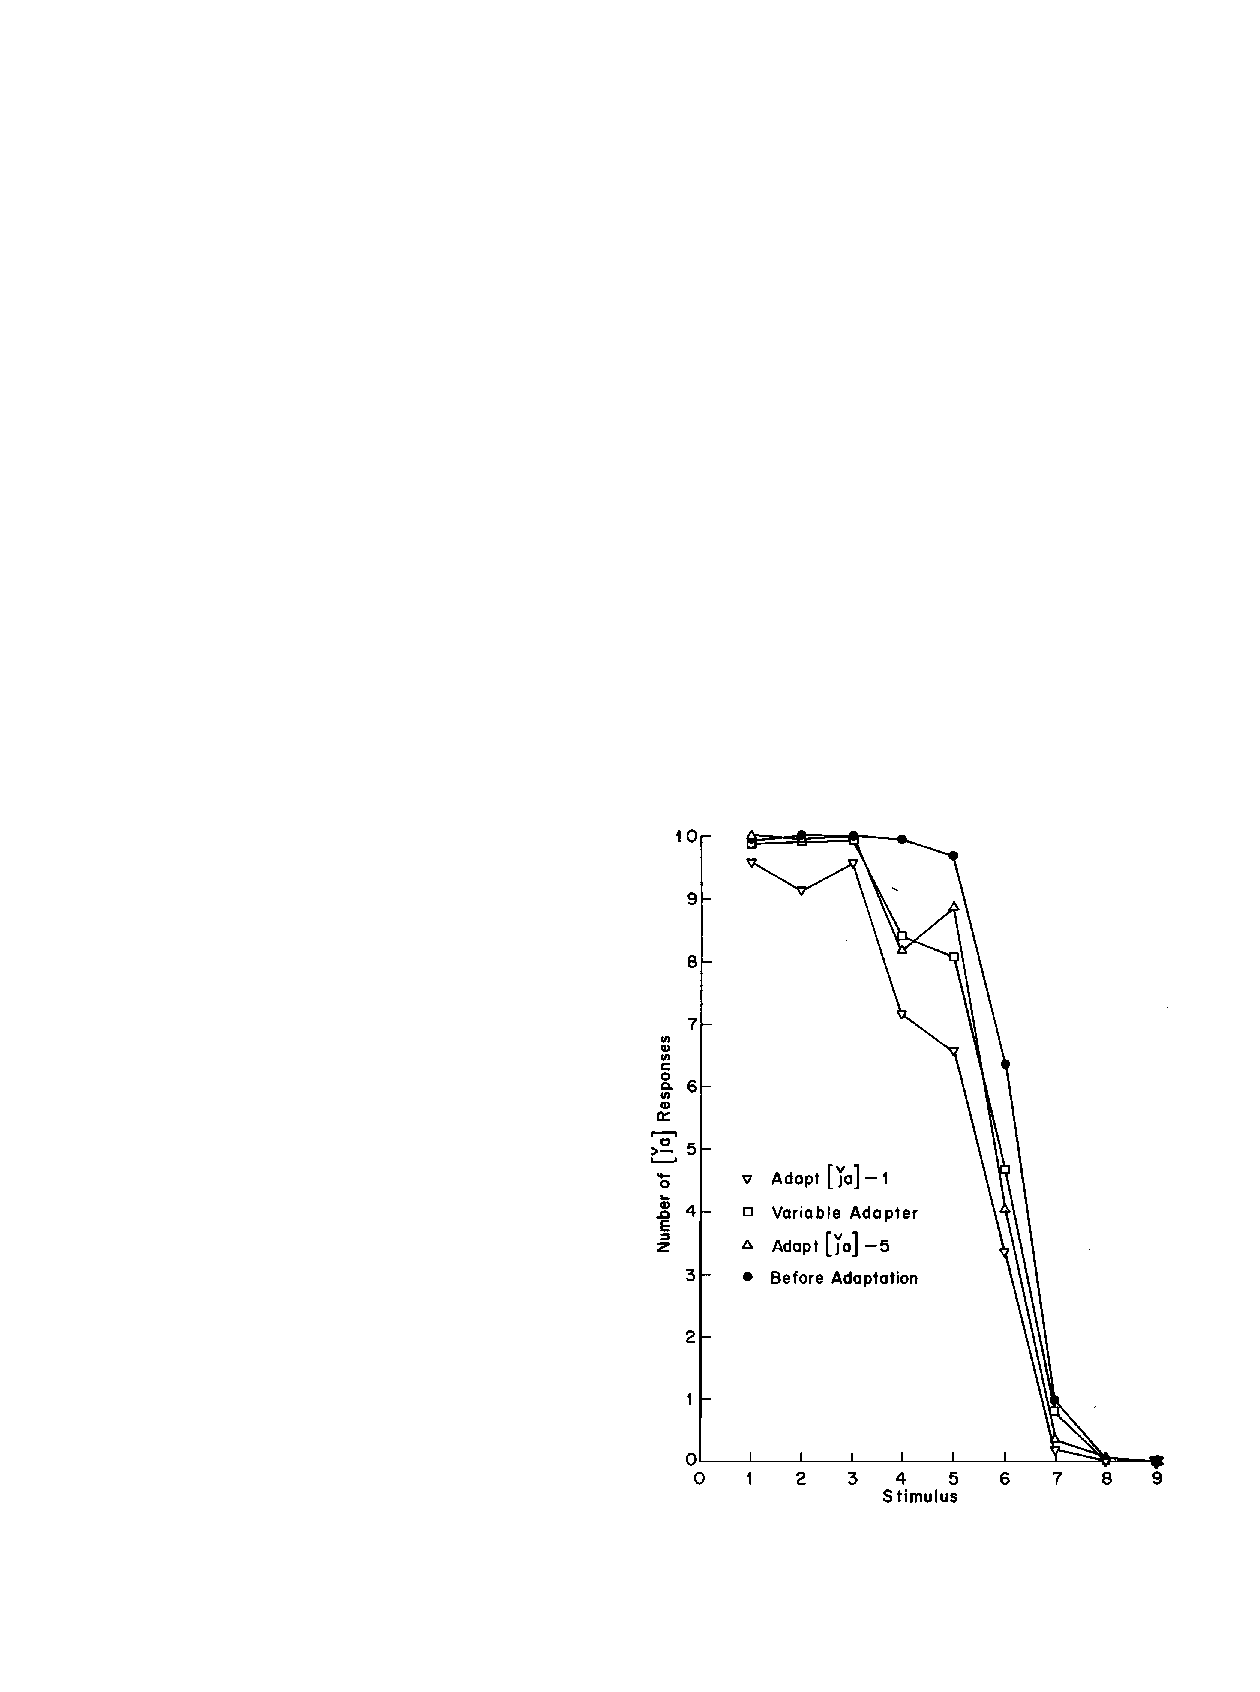
\includegraphics[width=0.5\textwidth]{cole-cooper-1977-fig3.pdf}
  \caption{Selective adaptation data from \protect\textcite{Cole1977}.  The $x$-axis shows the test stimuli on a 1 to 9, \ph{dZ} (the ``j'' sound in \emph{jump}) to \ph{d} continuum, and the $y$ axis shows subjects' average number of \ph{dZ} responses out of 10 repetitions of each test stimulus.  The ``variable adapter'' condition was exposure to a uniform distribution of stimuli, from $x=1$ to 6. Reproduced with permission from \protect\textcite{Cole1977}.}
  \label{fig:cole-1977-range-fixed-adaptors}
\end{figure}

In a similar vein, \textcite{Cole1977} investigated another type of distributional learning account, essentially assuming that listeners adapt only to changes in \emph{variance}. \citeauthor{Cole1977} referred to this as a ``narrowing of selectivity''. Based on data from several perception experiments, shown in Figure~\ref{fig:cole-1977-range-fixed-adaptors}, \citeauthor{Cole1977} concluded that narrowing of selectivity alone is not sufficient to explain selective adaptation.  If selective adaptation was caused by only adaptation to changes in category variance, than exposure to a range of adaptor stimuli with normal levels of variance should produce no selective adaptation at all.  However, \textcite{Cole1977} found that their ``variable'' adaptation condition (Figure~\ref{fig:cole-1977-range-fixed-adaptors}, squares) produced a negative after-effect just as large as a non-variable condition with a single, intermediate adaptor (Figure~\ref{fig:cole-1977-range-fixed-adaptors}, upward pointing triangles).

\label{r2-whole-distribution-3}
While this result cannot be explained in terms of adaptation to changes in variance alone, it is compatible with an ideal adapter.  Recall that the ideal adapter predicts that listeners are sensitive to the whole distribution of cues (including the \emph{mean}), not just the variance alone.  All else being equal, distributional learning predicts that a high-variance adaptor distribution will produce a smaller negative after-effect than a low-variance distribution, but all else is not equal in \textcite{Cole1977}.  The intermediate \ph{dZ} adaptor ($x=5$) was substantially farther from the \ph{dZ} endpoint ($x=1$) than the average of the variable-\ph{dZ} condition ($\bar x = 3.5$, a difference of $2.5$ from the endpoint, vs. a difference of 4 for the intermediate adaptor).\footnote{The same argument holds when using frication duration---the actual physical dimension manipulated to construct the continuum---instead of continuum step, with one caveat: due to an error in constructing the stimuli \autocite[Footnote 1]{Cole1977}, steps $x=4$ and $x=5$ both had frication durations of \SI{32}{\milli\second}, which means that the variability of the range condition is actually even lower than intended.}  An adaptor closer to the category prototype is, in a distributional learning model, predicted to produce a \emph{stronger} negative after-effect.  This would mitigate the effect of the higher variance in the range condition, which could explain why the intermediate and range conditions produce comparable effects.  In fact, the ideal adapter model qualitatively predicts that the low-variance, intermediate adaptor should lead to a slightly steeper category boundary, which is in fact what \textcite{Cole1977} appear to have found (see Figure~\ref{fig:cole-1977-range-fixed-adaptors}, $x=5,6,7$).


\subsection{Selective adaptation to audiovisual adaptors}
\label{sec:select-adapt-audi}

One prediction of a distributional learning theory of selective adaptation is that adaptation should depend on the joint distribution of all relevant cues, including visual speech cues.  However, studies using audiovisual adaptors \autocite{Roberts1981,Saldana1994} have been argued to support the view that selective adaptation is due to the fatigue of specifically \emph{auditory} feature detectors.  These audio-visual adaptors had large, categorical mismatches, which are intended to produce a McGurk Effect percept, where the perceived category of the audiovisual stimulus is different than the auditory component alone \autocite{McGurk1976}.  \textcite{Saldana1994} used an audio-\ph{ba}, visual-\ph{va} adaptor stimulus which was consistently identified as \ph{va} by participants.  This adaptor produced an after-effect on a \ph{ba}-\ph{va} continuum the same size as when the audio \ph{ba} component was presented separately.  \textcite{Saldana1994} interpreted this after-effect as evidence that listeners adapted to the audio component alone, rather than the integrated percept of \ph{va}.\footnote{An earlier study \protect\autocite{Roberts1981} used an audio-\ph{ba}, visual-\ph{ga} adaptor.  This was intended to produce a percept of \ph{da} \protect\autocite[as in][]{McGurk1976}, but only half of their subjects perceived an alveolar sound at all, with the others reporting \ph{kl}, \ph{m}, or \ph{fl} \protect\autocite{Saldana1994}.  This makes it difficult to interpret their results and so we do not discuss them further here.}  As a result, \textcite{Saldana1994} rejected explanations of selective adaptation as learning at the level of phonetic categories---as in distributional learning---in favor of a process of purely low-level acoustic feature detector fatigue.

However, it is not possible to tell whether the observed effect was due to selective adaptation of \ph b (lower \ph b variance), or \emph{recalibration} of \ph v (shift in \ph v mean), since both would produce a shift in the category boundary towards \ph b.  Unless they completely ignored the audio component, subjects in this experiment likely perceived the audio-visual adaptor not as a perfect \ph{va}, but rather a somewhat \ph{ba}-like \ph{va}.  \textcite{Kleinschmidt2011} presented evidence that phonetic distributional learning operates on this kind of combined audio-visual percept \autocite[also cf.][]{Bejjanki2011,Ernst2004}.  If this is in fact the case, then listeners in \citeauthor{Saldana1994}'s experiment should update their beliefs about the \ph v cue distribution, shifting it to be more \ph b like.  The result of this recalibration of \ph v would be more \ph v and hence fewer \ph b responses, which is the after-effect that \textcite{Saldana1994} observed.  Thus, the results of \textcite{Saldana1994} are not \emph{necessarily} incompatible with distributional learning at the phonetic category level. 

We believe that future work addressing this question will prove particularly valuable in evaluating the feasibility of an explanation of selective adaptation purely in terms of distributional learning. For instance, we have suggested that the after-effects observed by \textcite{Saldana1994} are due to \emph{recalibration} to an integrated percept that combines audio and visual cues.  This account predicts that changing the reliability of the \emph{visual} cue should change the integrated percept \autocite[as observed by][]{Bejjanki2011,Ernst2004}, and thus the resulting after-effect, while the audio-only selective adaptation account offered by \textcite{Saldana1994} predicts that changing the visual cue should have no effect at all.


\section{Discussion}
\label{sec:discussion}

Since selective adaptation for speech was first discovered, our understanding of both adaptation in sensory systems in general, and flexibility in the language system in particular has come a long way.  First, work on non-linguistic sensory adaptation has established that adaptation goes far beyond fatigue of feedforward feature detectors \autocite{Brenner2000,Dragoi2000,Fairhall2001,Gutfreund2012,Kohn2004,Kohn2007,Sharpee2006,Webster2005}.  In particular, there is tentative evidence that sensory adaptation serves to increase the efficiency of the representation of sensory information, based on the statistical or distributional properties of recent sensory input.  Second, the speech perception system is now understood to be flexible in smart ways, for example, by recalibrating phonetic categories based on unusual pronunciations \autocite{Bertelson2003,Kraljic2005,Norris2003}.

Both of these developments are rooted in a growing awareness of the importance of distributional or statistical properties of the sensory world for understanding sensory systems.  While these two developments may appear rather dissimilar---one concerned with the allocation of scarce neural resources, and the other with robust language comprehension in the presence of variability---they come together in the phenomenon of phonetic selective adaptation. Although for different reasons than originally anticipated, selective adaptation thus rightly deserves the spotlight it enjoyed in the early era of cognitive research on speech perception.  Moreover, we have tentatively proposed that selective adaptation can be understood as one consequence of the more general process of distributional learning, along with phonetic recalibration and other forms of smart adaptation in language processing \autocite{Kleinschmidt2015}.  This proposal provides good coverage of the data that exists on how selective adaptation changes listeners' classification of speech sounds.

More importantly, however, we hope that this proposal will provide a road map for how specifically to go about re-evaluating selective adaptation.  There is a great deal of work that is required to flesh out and critically evaluate such a distributional-learning theory.  In closing, we discuss four important directions for future research.

\subsection{Future directions}
\label{sec:future-directions-1}

First, distributional learning is a computational-level account, in the sense of \textcite{Marr1982}.  Such accounts focus on the in-principle constraints on a cognitive system that come from the information that is available and the task the system is carrying out.  While these considerations guide and constrain cognitive models, they are not cognitive models per se.  There are many different possible algorithms, processes, or representations that can carry out the \emph{computation} of distributional learning, and many possible neural implementations for each of those.  Fleshing out the relationships between these is an important next step in formulating and evaluating a complete distributional learning theory of selective adaptation.  Critically, mechanistic- and computational-level explanations are not necessarily in opposition.  It may well be the case, for instance, that a population of fatiguing feature detectors can approximate distributional learning in some circumstances.  These links are, however, largely un-explored, and call for future work.

Second, and relatedly, we have focused on the effects of selective adaptation on listeners' \emph{classification} decisions, and have not discussed reaction time effects of selective adaptation.  Such effects are well-documented \autocite{Samuel1986,Samuel1996} and historically one of the most important sources of insight into selective adaptation.  Across the cognitive sciences, the \emph{outcome} of a decision can often be dissociated from the \emph{time course} of that decision \autocite[see, e.g., the related discussion for lexical selection in speech production;][]{Mahon2007,Oppenheim2010}.  The same is true in phonetic selective adaptation: two adaptors can produce the same boundary shifts, but different changes in reaction time \autocite{Samuel1996}.  A computational-level account like distributional learning naturally captures the decisions that listeners make, but the time course falls more under the purview of process- or implementation-level accounts.  Thus, a critical next step in evaluating distributional learning as a theory of adaptation in speech perception (and perception more broadly) is to develop proces- and implementation-level models that carry out the computations  of distributional learning.  There is some promising if preliminary work that links increased probability of a stimulus to an increase in signal-to-noise ratio in sensory representations \autocite{Stocker2006,Wei2012}.  Increased reaction times might be a consequence of achieving such increased signal-to-noise ratio through, for instance, stronger lateral inhibition leading to sparser responses by effectively narrowing receptive fields \autocite{Gardner2004}.  We emphasize that this is only one possibility, and that in general linking distributional learning to reaction time data at all is a critical direction for future work.

Third, as we have outlined it here, distributional learning accounts for selective adaptation through changes in listeners' beliefs about the \emph{variance} of the adapted phonetic category.  There is some evidence that listeners are, in fact sensitive to category variance \autocite{Clayards2008,Cole1977,Newman2001,Schreiber2013}, but only a few studies have explored this systematically.  Only one study that we know of has specifically investigated the link between category variance and selective adaptation \autocite{Cole1977}, and while, as we have argued, their results are consistent with a distributional learning theory, their design confounds category variance and category \emph{mean}.  More work is required, first to determine what distributional learning predicts the effect of different degrees of category variance is, and second to see whether listeners actually behave in the predicted ways.

Fourth, distributional learning provides a bridge between selective adaptation---typically thought of as a low-level process---and higher-level processes like talker-specific recalibration and accent adaptation.  A hallmark of these processes is that listeners often apply what they have previously learned to future situations in smart ways.  This can mean \emph{recognizing} a previously encountered talker, as demonstrated by recalibration that persists even after 12 hours outside the lab \autocite{Eisner2006}.  It can also mean \emph{generalizing} learning to an unfamiliar talker that is similar to previously-encountered talkers, as demonstrated by talker-independent accent adaptation \autocite{Bradlow2008}.  Elsewhere \autocite{Kleinschmidt2015}, we have proposed that such cross-situational learning effects can be modeled as distributional learning that is indexed to particular indexical variables like a talker, groups of talkers, or environment.  Such hierarchical distributional learning enables previously learned cue distributions to be re-learned very quickly when the associated indexical variable is encountered again \autocite[for similar arguments applied to domain-general sensory/motor learning, see][]{Qian2012,Qian2013}.  If selective adaptation is due to the same sort of distributional learning, then it follows that listeners should re-adapt to previously encountered distributions more quickly than the initial adaptation.  To our knowledge, this prediction has not been addressed in the literature on phonetic selective adaptation.


\subsection{Whither feature detectors?}
\label{sec:whith-feat-detect}

We have focused on---and argued against---the assumption that phonetic selective adaptation is the \emph{fatigue} of auditory-phonetic feature detectors, without discussing the nature or existence of these feature detectors themselves.  The early work on selective adaptation was rightly criticized for relying on problematic assumptions about these feature detectors \autocite{Remez1987}: that there were a small number of them, specified largely a priori, which respond largely independently of context, and are organized into clearly delineated layers (simple acoustic, complex acoustic, phonetic, etc.).  Our proposal that selective adaptation be seen as a form of distributional learning does not rely on these same assumptions.  Nevertheless, a fully fleshed out theory of adaptation as distributional learning has to say something about what those distributions are \emph{of}.  The things that these distributions cover may be seen as a sort of features, and expressing those distributions in terms of some relatively low-dimensional compression of the full acoustic input information makes sense for the same reasons that distributional learning makes sense: sensory systems have limited representational resources, and care about some aspects of the sensory world more than others.  But there is no guarantee that these ``features'' will line up with our intuitions about what the relevant features are, or that they will be organized in clearly delineated levels.  

There is also no guarantee that adaptation itself provides a straightforward means of probing these features.  In fact, the work on visual adaptation we reviewed here suggests that adaptation has to be considered in terms of distributions across \emph{multiple levels} simultaneously.  We take these levels to refer not only to part-whole feature relationships \autocite{He2012}, but also to the statistical sense of distributions over the same features but at different time scales (seconds vs. minutes) \autocite{Chopin2012} or groups of situations (talker, accent, language, etc.). There is analogous work in speech perception, including selective adaptation, that makes the same point \autocites[e.g., adaptation of single segments depends on the syllabic context][]{Bryant1978}[and others summarized in][]{Remez1987}, but the consequences of adaptation across multiple levels have not been fully explored, either in vision or speech perception.


\subsection{Speech as a model organism for perception}
\label{sec:speech-as-model}

Finally, we close by arguing that selective adaptation provides a good bridge between speech perception and the study of perception more generally.  As we have discussed, recent work on general sensory adaptation has revealed that adaptation has a variety of functional properties that make it interesting as an object of study in its own right, rather than just a methodological tool.  The emerging computational understanding of adaptation puts it squarely at the intersection of many fundamental and interesting questions in the study of perception, such as the interaction between bottom-up and top-down information, the ways that innate constraints and information from the world shape perceptual systems, the role that probabilistic predictions play in perception \autocite[e.g.,][]{He2012}, and how the brain manages to process sensory information efficiently in a variable world with a limited stock of representational resources, among others.  

Speech perception exemplifies many of these issues as well as, or better than, other perceptual processes.  As a sensory signal, speech is structured in multiple, intersecting ways.  On the one hand, there is the \emph{linguistic} structure of speech: individual sounds combine into phonetic categories, categories into words, words into phrases, phrases into sentences, etc.  On the other hand, there is the \emph{indexical} structure of speech: every talker maps phonetic categories to sounds in a different way, often dramatically so, and talkers themselves can be clustered based on dialect, native language background, etc.  While neither sort of structure is exhaustively understood, they are understood well enough to manipulate them experimentally in ways that carefully control their statistical properties but are reasonably ecologically valid \autocite{Allen2004,Clayards2008,Newman2001}.  This stands in contrast to visual psychophysics, which in large part relies on simple, artificial stimuli in order to achieve careful control.  Obviously, much has been learned from these techniques.  But for investigating questions of how sensory systems deal with changes in the statistics of the sensory world, more leverage might be provided by studying sensory domains where such deviations occur frequently and are typically managed successfully by human observers.  Speech perception is just such a domain: differences between talkers are well-studied, often to the extent of quantifying the statistical deviations from one talker to another.  Likewise, the last decade has seen an explosion in research showing listeners can rapidly adapt to different talkers.

What role does phonetic selective adaptation play in all of this?  It sits at the intersection of the study of low-level adaptation in vision and more recent work on smart plasticity in speech perception and language comprehension.  It is our hope that, by bringing new attention to the long literature on phonetic selective adaptation, researchers studying speech perception will be more aware of developments in how sensory adaptation more broadly is understood, and that researchers who study perception in general will consider both the potential offered and the challenges posed by speech perception as a perceptual process.

\subsection{Conclusion}
\label{sec:conclusion}

The literature on phonetic selective adaptation is long, complex, and often apparently contradictory \autocites[as summarized by][]{Samuel1986}[and][]{Remez1987}.  Over time, interest in the theoretical basis for this fundamental phenomenon has dwindled.  We believe, though, that adaptation is an important property of perception in general, and of speech perception in particular, and that this literature deserves more attention. Recent developments in the understanding of sensory adaptation more broadly and flexibility in speech perception in particular challenge some of the basic assumptions of early work on phonetic selective adaptation.  However, as we have argued, they also provide a set of conceptual tools for understanding phonetic selective adaptation in the broader context of language comprehension and sensory adaptation.  We have proposed, to start, that selective adaptation can be seen as a form of distributional learning.  Distributional learning provides a coherent perspective on the existing literature on phonetic selective adaptation, highlights parallels with non-speech adaptation, and suggests a unifying perspective on flexibility in adult language comprehension.  It also, most importantly, raises a number of interesting questions for future work.

